% Copyright 2023 by Marcos Laureano (marcos.laureano@ifpr.edu.br)
% This file may be distributed and/or modified
%
% 1. under the LaTeX Project Public License and/or
% 2. under the GNU Public License.
%
% Original from Marco Barisione 


\documentclass{beamer}
\usetheme[pageofpages=de,% String used between the current page and the
                         % total page count.
          bullet=circle,% Use circles instead of squares for bullets.
          titleline=true,% Show a line below the frame title.
          alternativetitlepage=true,% Use the fancy title page.
          titlepagelogo=LaRCA,% Logo for the first page.
          watermark=LaRCA_semifpr.png,% Watermark used in every page.
          watermarkheight=50px,% Height of the watermark.
          watermarkheightmult=4,% The watermark image is 4 times bigger
                                % than watermarkheight.
          ]{LarCA} 
          
          


\usepackage[utf8]{inputenc}
\usepackage[brazilian]{babel}
\usepackage{animate}
\usepackage{url,hyperref}

\author{Marcos Laureano\\marcos.laureano@ifpr.edu.br}
\title{STEAM -- Robótica Educacional $\times$ Robótica de Competição}
\subtitle{Estamos fazendo da forma certa?}
\institute{Laboratório de Robótica e Computação Aplicada do Campus Pinhais -- Instituto Federal do Paraná}
\date{\today}

\begin{document}
\begin{frame}[t,plain]
\titlepage
\end{frame}

\AtBeginSection[]
{
  \setcounter{tocdepth}{2}
  \begin{frame}
   \frametitle{Sumário}
   \tableofcontents[currentsection, hideothersubsections]
  \end{frame}
}



\section[Sumário]{}
\frame{\tableofcontents}

\section{Introdução}

\begin{frame}
\frametitle{Antes de começar!}
\framesubtitle{}
   \begin{block}{Eu não vim aqui}
   Tecer críticas ao trabalho desenvolvido! Questionar as políticas de educação!
   Ou mesmo falar que o foi feito está errado!
   \end{block}
   \begin{block}{Eu vim aqui}
   Para quebrar paradigmas! Mostrar novos caminhos! E colaborar com os meus mais de 10 anos nessa área (e aprendo coisas novas todos os dias)!
   \end{block}
\end{frame}

\subsection{STEAM -- Science, Tecnology, Enginnering, \emph{Arts} and Matematics}

\begin{frame}
\frametitle{Ciência, Tecnologia, Engenharia, Arte e Matemática}
\framesubtitle{}
   \begin{block}{STEM}
   Simboliza uma abordagem moderna da ciência e assuntos relacionados, com foco na resolução de problemas por meio do pensamento crítico e das habilidades analíticas.
   \end{block}
   \begin{block}{Porém}
   conhecimentos de engenharia,tecnologia, ciências e matemática não podem nos ajudar a ressuscitar a educação sozinhos.
   \end{block}
   \begin{block}{STEAM}
   Explora os mesmos assuntos, mas incorpora o pensamento criativo e as artes aplicadas ao ensino e a situações reais.
   \end{block}
\end{frame}

\begin{frame}
\frametitle{STEAM}
\framesubtitle{Compilação de cinco campos acadêmicos}

\begin{columns}
	  \column{.40\textwidth}
\begin{flushright}
    \includegraphics[width=4.5cm]{imagens/6617}
\end{flushright}

	  \column{.60\textwidth}

	\begin{block}{Abordagem educacional}
	Para ensinar e aprender disciplinas STEM por meio das artes. Basicamente, intencionalmente integra estudos acadêmicos com disciplinas artísticas, por exemplo, artes visuais, dança, música e teatro.
	\end{block}
	
\end{columns}
\end{frame}

\subsection{Artes aplicadas ao ensino e a situações reais}
\begin{frame}
\frametitle{Artes aplicadas ao ensino e a situações reais}
\framesubtitle{}
	\begin{block}{A arte e seus processos de pensamento criativos}
	São um parceiro necessário para completar o tipo de aprendizado que queremos que nossos filhos experimentem.
	\end{block}

	\begin{block}{Transformar o STEM em STEAM}
	É uma maneira de garantir que envolvamos nossos alunos em uma educação que os compele, desafie e os inspire.
	\end{block}
	
	\begin{block}{Arte é descobrir e criar maneiras engenhosas de resolver problemas, integrar princípios e apresentar informações.}
	Ao adicionar o elemento da arte ao pensamento baseado em STEM, os educadores acreditam que os alunos podem usar os dois lados do cérebro - analítico e criativo - para desenvolver os melhores pensadores de amanhã.
	\end{block}
\end{frame}

\section{Robótica Educacional}

\subsection{O que NÃO é!}
\begin{frame}
\frametitle{A verdade é triste!}
\framesubtitle{}
	\begin{block}{Não é apenas ensinar sobre componentes}
	Mas fazer o aluno pensar e relacionar com as demais questões ao seu redor.
	\end{block}
	
	\begin{block}{Exemplo clássico -- pisca LED com Arduíno}
		\begin{itemize}
			\item Fala para pegar um resistor -- sem explicar o motivo direito;
			\item Sempre usa um LED vermelho -- e nem sabe o motivo;
			\item Conecta em uma porta de algum tutorial na internet -- 11 é sempre comum, mas ninguém explica as implicações;
			\item Baixa o programa do tutorial e \emph{voilà}!!
		\end{itemize}
	\end{block}
	
\end{frame}

\subsection{O que deveria ser!}

\begin{frame}
\frametitle{Um exemplo com STEAM}
\framesubtitle{Física e eletrônica básica e artes envolvidas}
	\begin{columns}
	   \column{.40\textwidth}
	  \animategraphics[loop,autoplay,width=1\linewidth]{20}{./imagens/RGB/RGB_animado-}{0}{306}
	  \column{.60\textwidth}
	  	\begin{block}{Pisca LED}
		\begin{itemize}
			\item Fazer relação com luz emitida (padrão RGB) e luz absorvida (padrão CMYK);
			\item Explicar que leds de cores diferentes usam voltagens diferentes -- LED Azul e brancos não precisam de resistores pois funcionam em $\approx 3$ volts;
			\item Explicar que se usam as portas digitais do Arduíno (2 -- 13) para leds;
		\end{itemize}
		\end{block}
	\end{columns}
\end{frame}


\begin{frame}
\frametitle{Exemplo STEAM com sensor de Luminosidade}
\framesubtitle{Física básica -- Luz ambiente $\times$ Refletida}
	\begin{columns}
	   \column{.65\textwidth}
		\begin{block}{Explicar como os sensores funcionam}
			\begin{itemize}
				\item A diferença é qual o tipo de luz que o sensor fará a leitura;
				\item No caso da função luz ambiente, a leitura terá o valor da luz que vem de todos os lados, ou seja, de todo o ambiente no qual o robô está;
				\item Na função luz refletida, a leitura sofre menos influência da iluminação do ambiente, pois o próprio sensor se encarrega de fornecer a luz, através de um LED vermelho, que fica ligado.
			\end{itemize}
		\end{block}
	\column{.35\textwidth}
	\begin{flushright}
	

    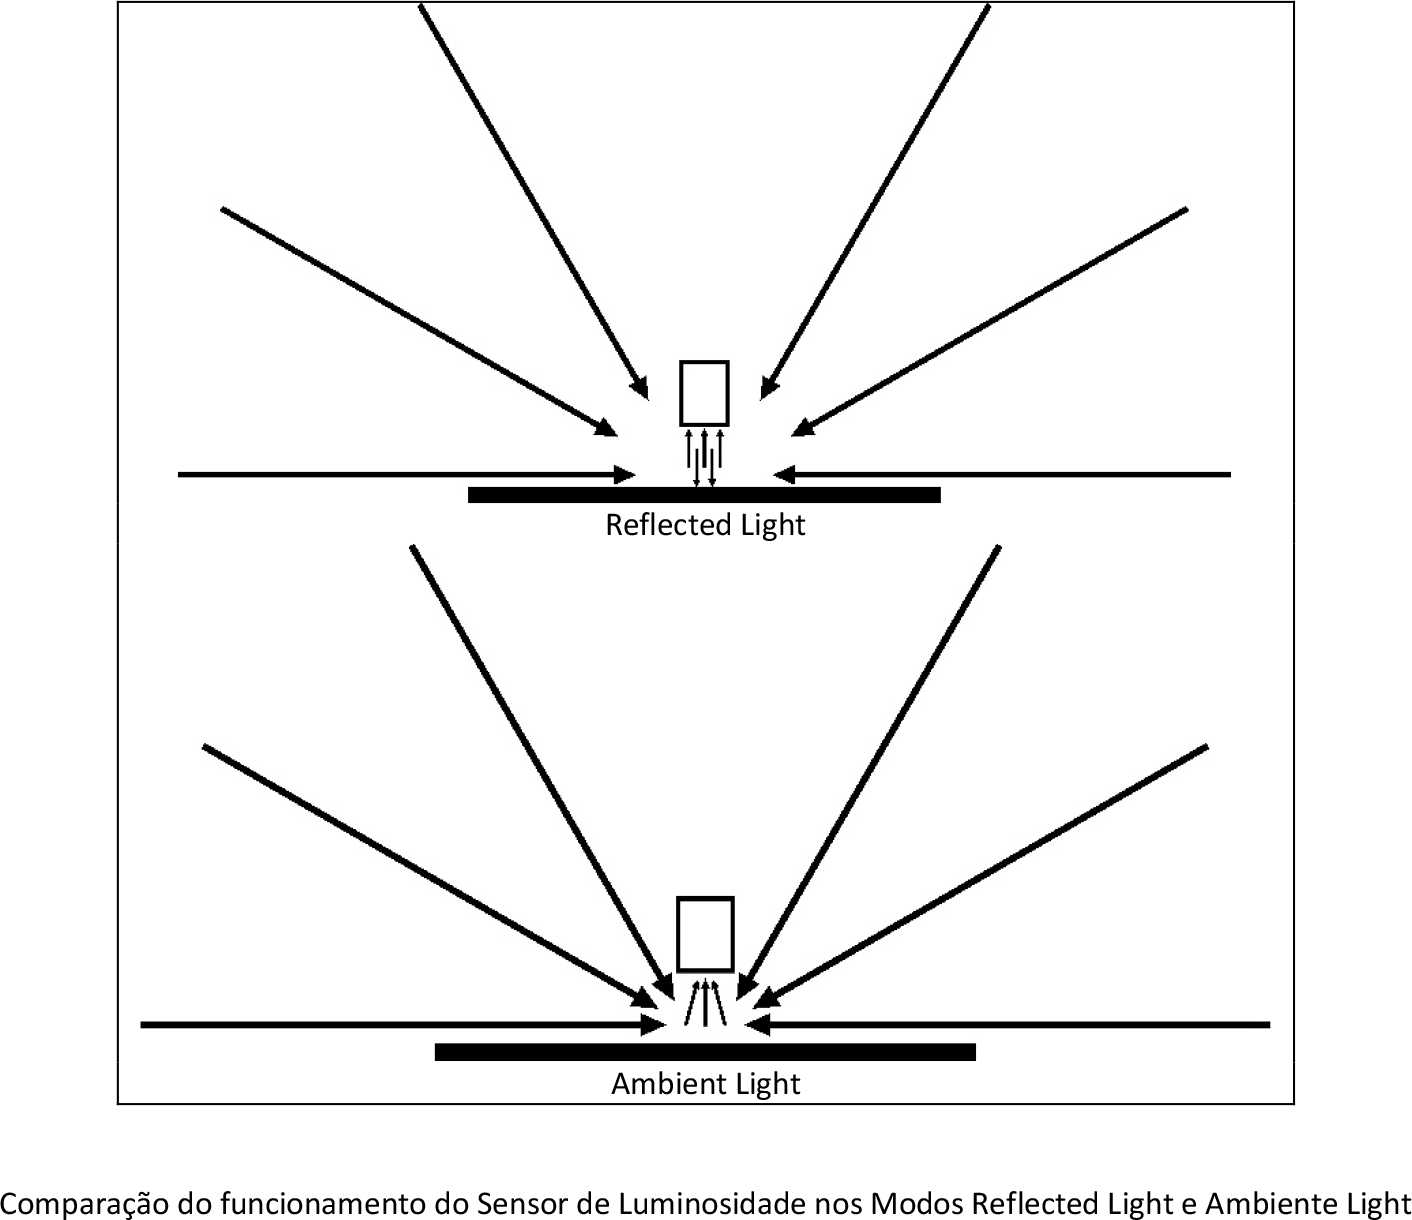
\includegraphics[width=1.1\textwidth]{imagens/sensor_cor}
	\end{flushright}
	\end{columns}
\end{frame}

\begin{frame}
\frametitle{Exemplo STEAM com sensor ultrassônico}
\framesubtitle{Façam experimentos!!!!!!}

		\begin{block}{Explicar como os materiais alteram o funcionamento do sensor -- distância real 11,5 cm.}
			\begin{itemize}
				\item Garrafa d'água (cheia) -- 11,4 cm;
 				\item Garrafa d'água (vazia) -- alternando entre 11,2 e 11,4 cm (alguém sabe o motivo? Eu sei...);
 				\item Caixa de papelão -- 10,1 cm;
 				\item Livro -- 10,7 cm;
 				\item Folhas de papel (5 folhas) -- 10,3 cm;
 				\item Pasta de plástico (apenas 1 lado) -- 10,7 cm;
 				\item Pasta de plástico (2 lados) -- 11,4 cm;
 				\item Parede de tijolos -- 10,9 cm.
 			\end{itemize}
		\end{block}
\end{frame}

\begin{frame}
\frametitle{Exemplo com mecanização}
\framesubtitle{Rodas influenciam o funcionamento do robô!}
	\begin{columns}
	   \column{.33\textwidth}
	   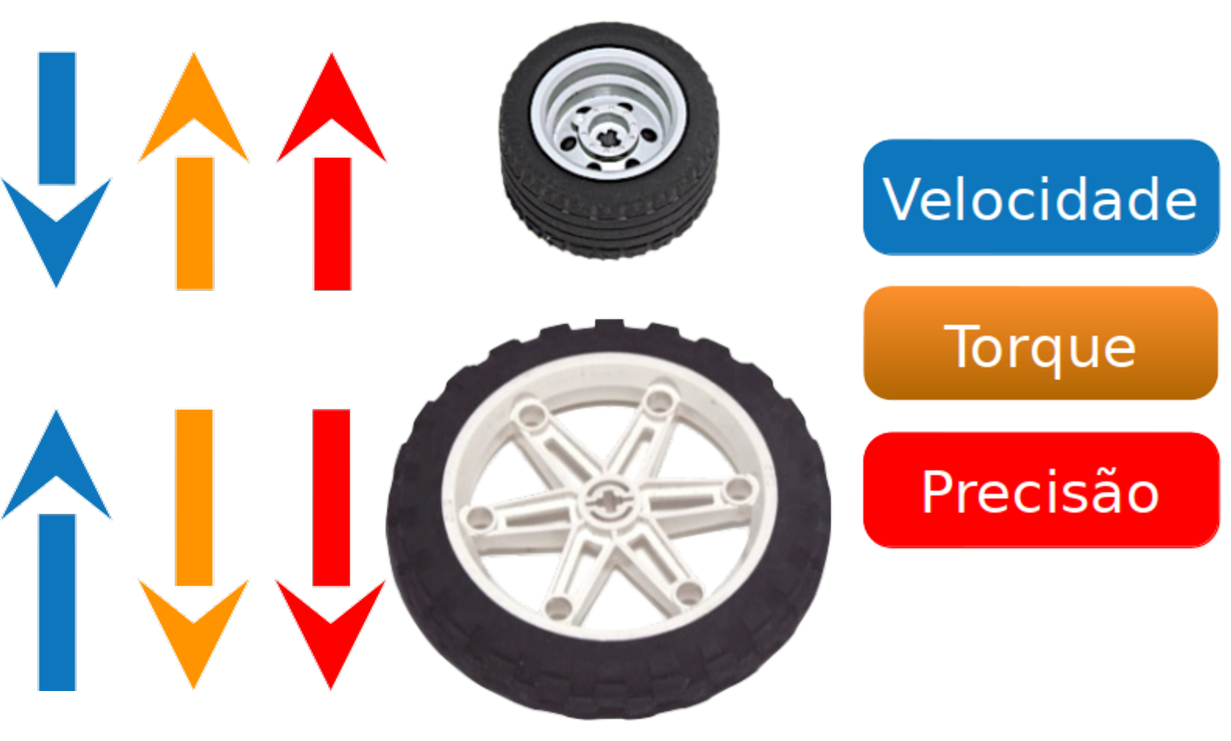
\includegraphics[width=1\textwidth]{imagens/escolha_roda_tamanho}
       \column{.33\textwidth}
       	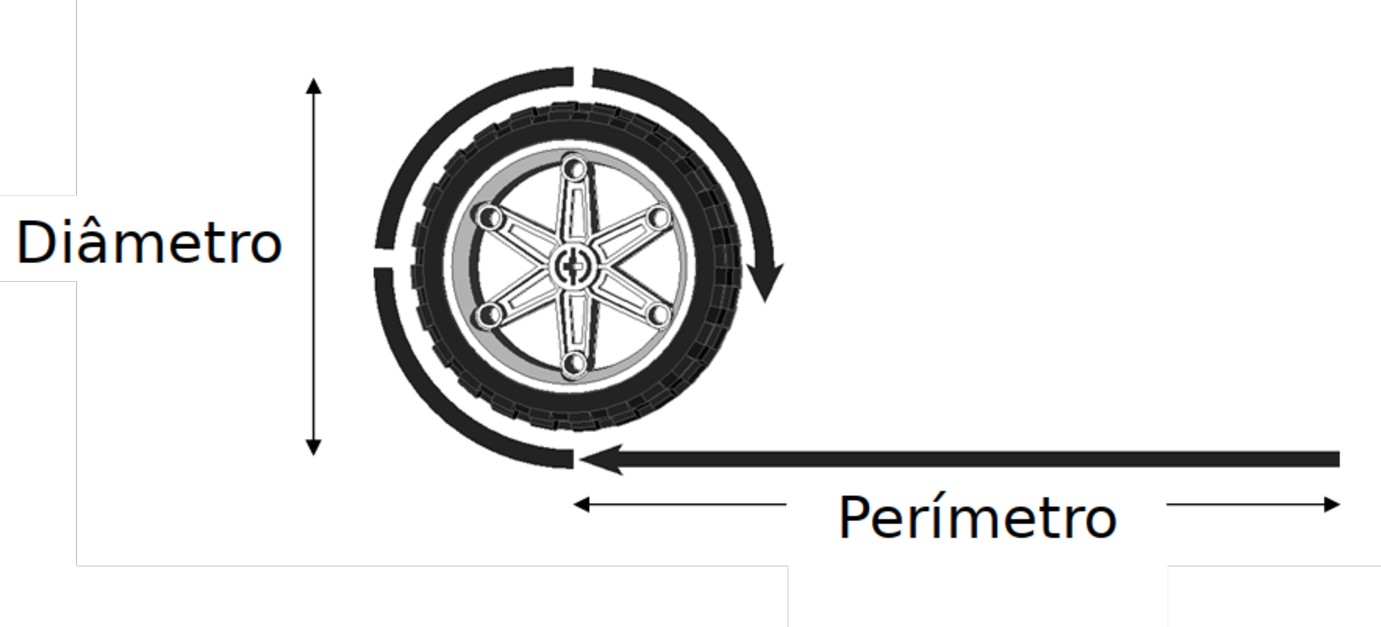
\includegraphics[width=1\textwidth]{imagens/escolha_roda_perimetro}
       \column{.33\textwidth}
       	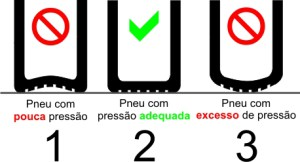
\includegraphics[width=1\textwidth]{imagens/pressao_pneu_inadequado}
    \end{columns}
\end{frame}


\section{Robótica de Competição}

\subsection{O que é}

\begin{frame}
	\frametitle{Robótica de competição}
	\framesubtitle{Um campo emocionante onde equipes constroem e programam robôs para competir em eventos ou desafios.}
	\begin{block}{Podem variar desde competições de combate entre robôs}
		Até desafios de resolução de problemas ou tarefas específicas. 
	\end{block}
	
	\begin{block}{As competições podem ser organizadas em várias categorias}
		\begin{itemize}
			\item Combate de Robôs;
			\item Robótica de Resgate;
			\item Desafios de Tarefas Específicas;
			\item Robótica Educacional.
		\end{itemize}
	\end{block}

\end{frame}

\begin{frame}
	\frametitle{Falando sobre os tipos de competição}
	\framesubtitle{Competições organizadas anualmente no Salão de Robótica em Curitiba com apoio do LaRCA}
	\begin{block}{Combate de Robôs}
		Os robôs são projetados para competir em arenas, buscando incapacitar ou empurrar seus oponentes para fora da área de combate.
		\linebreak
		\linebreak
		Exemplos: UFC de Robôs e Sumô.
	\end{block}
	\begin{block}{Robótica de Resgate}
		Envolvem robôs que precisam navegar por um ambiente simulado para encontrar e resgatar vítimas ou cumprir certos objetivos em cenários de desastres.
		\linebreak
		\linebreak
		Exemplo: OBR -- Olimpíada Brasileira de Robótica.
	\end{block}

\end{frame}

\begin{frame}
	\frametitle{Falando sobre os tipos de competição}
	\framesubtitle{Competições organizadas anualmente no Salão de Robótica em Curitiba com apoio do LaRCA}
	\begin{block}{Desafios de Tarefas Específicas}
		Eventos onde os robôs são testados em realizar tarefas específicas, como percorrer um labirinto, resolver quebra-cabeças ou executar atividades industriais.
		\linebreak
		\linebreak
		Exemplos: Seguidor de linha e Trekking.
	\end{block}
	\begin{block}{Robótica Educacional}
		Competições voltadas para estudantes, que visam promover o aprendizado STEM, incentivando a construção e programação de robôs.
		\linebreak
		\linebreak
		Exemplo: FLL -- First Lego League.
		
		Organizado e operado pelo SESI.
	\end{block}
\end{frame}

\subsection{Importante}
\begin{frame}
	\frametitle{Importante}
	\framesubtitle{Qualquer competição de robótica pode ser aplicada STEAM}
	\begin{block}{Aprendizado de física e química}
		Ao verificar o ambiente que cerca a competição.
	\end{block}

	\begin{block}{Aprendizado de matemática e engenharia}
		No processo de construção e programação do robô.
	\end{block}

	\begin{block}{Aprendizado de Artes}
		Existem premiações específicas para robôs mais bonitos e até uma categoria específica chamada dança de robôs (\emph{on stage}).
	\end{block}

	\begin{block}{Habilidades Sociais}
		Trabalhar em equipe, respeitar os valores sociais e humanos, ciências humanas.
	\end{block}

\end{frame}

\begin{frame}
	\frametitle{Qualquer competição de robótica pode ser aplicada STEAM}
	\framesubtitle{}


	\begin{block}{Habilidades de Escrita}
		Documentação de projetos, escrever artigos.
		\linebreak
		\linebreak
		Esse, talvez, seja um dos mais importantes e que precisam ser desenvolvidos pelos nossos alunos. Atualmente eles escrevem cada vez menos a ponto de terem dificuldades de compreensão de texto, leitura e escrita.
	\end{block}

	\begin{block}{O céu é o limite}
		E basta dar um passo de cada vez -- nem tudo precisa ser feito de uma vez só.
	\end{block}

\end{frame}

\subsection{Competições de robótica educacional -- Como o LaRCA pode ajudar}

\begin{frame}
	\frametitle{Competições de robótica educacional -- Como o LaRCA pode ajudar}
	\framesubtitle{Minha Experiência -- mas não sou o único no laboratório}
	\begin{block}{+10 de anos}
		\begin{itemize}
			\item Técnico -- bi-campeão da OBR com equipe exclusiva de meninas;
			\item Juiz de competição -- FLL, OBR, Futebol de Robôs, Sumô, UFC, etc$\dots$;
			\item Juiz chefe de evento -- FLL, OBR, etc$\dots$;
			\item Competidor -- Futebol de robôs -- nacional e internacional, inclusive com campeonato internacional;
			\item Organizador de evento -- Salão de Robótica, OBR, Mostra de Robótica, etc$\dots$
		\end{itemize}
	\end{block}

\end{frame}

\begin{frame}
	\frametitle{Em desenvolvimento}
	\framesubtitle{Apenas para citar alguns}
	\begin{block}{Especialização em Robótica Educacional}
		Semi-presencial (atividades teóricas online e práticas presenciais).
	\end{block}

	\begin{block}{Competições de drone}
		Parceria com a Petrobras.
	\end{block}

	\begin{block}{Ensino de Programação para crianças no ensino fundamental}
		Parceria com a Prefeitura Municipal de Pinhais (mais de 600 crianças e 80 professores em 2 anos).
	\end{block}

	\begin{block}{Bacharelado em Ciência da Computação}
		Focado em Robótica, Inteligência Artificial e Sistemas Distribuídos.
	\end{block}

\end{frame}

\begin{frame}
	\frametitle{Em desenvolvimento}
	\framesubtitle{Apenas para citar mais alguns}
	\begin{block}{Monitoramento de meio ambiente}
		Utilizando IoT -- Internet das coisas e aplicação de drones.
	\end{block}

	\begin{block}{Resgate de vítimas de afogamento utilizando sensores robóticos}
		Parceria com corpo de bombeiros.
	\end{block}

	\begin{block}{Implantação de incubadoras}
		Desenvolvimento de futuros unicórnios.
	\end{block}

	\begin{block}{Desenvolvimento de um robô educacional de baixo custo}
		Utilizado com Arduíno, ESP32, MicroBit, Pico--C3, Raspberry, etc$\dots$
		
		Nesse caso o professor escolhe a placa robótica que mais lhe agrada (e cabe no seu orçamento) e usa o material didático adaptado para cada situação.
		\end{block}
\end{frame}

\begin{frame}
	\frametitle{Em desenvolvimento -- esses para o próximo ano}
	\framesubtitle{Após retorno das férias}
	\begin{block}{Site do LaRCA}
		Com materiais e projetos disponíveis para download.
		
		\url{https://www.larca.org.br}
	\end{block}

	\begin{block}{Uma revista online com submissão aberta e publicação gratuita}
		Com revisão por pares, critérios para submissão e chamada permanente. Mas sem cobrar taxas de publicação.
		
		\url{https://journal.larca.org.br/}
	\end{block}

\end{frame}

\subsection{Alguns links de vídeos de competições}
\begin{frame}
   \frametitle{Alguns links de vídeos de competições}
   \framesubtitle{Se expirem}
   
   	\begin{block}{O que é o Salão de Robótica}
   		\url{https://www.youtube.com/watch?v=nf6GmBGTnj8}
	\end{block}

	\begin{block}{On Stage -- dança de robôs}
		\url{https://www.youtube.com/watch?v=T1qQKkiF64s}
	\end{block}
	
	\begin{block}{Resgate}
		\url{https://www.youtube.com/watch?v=44IZUZ5mNx8}
	\end{block}
	
	\begin{block}{Seguidor de linha}
		\url{https://www.youtube.com/watch?v=mBZU9S0kZJw}
		\url{https://www.youtube.com/watch?v=ijKpDYibkUs}
	\end{block}	

	\begin{block}{Futebol de Robôs}
	\url{https://www.youtube.com/watch?v=sZI2DS-OK4s}
	\end{block}	
	
	
\end{frame}

\section{Dúvidas}
\begin{frame}
   \frametitle{Se manifestem}
   \begin{columns}
	   \column{.60\textwidth}
	   \begin{flushright}
	   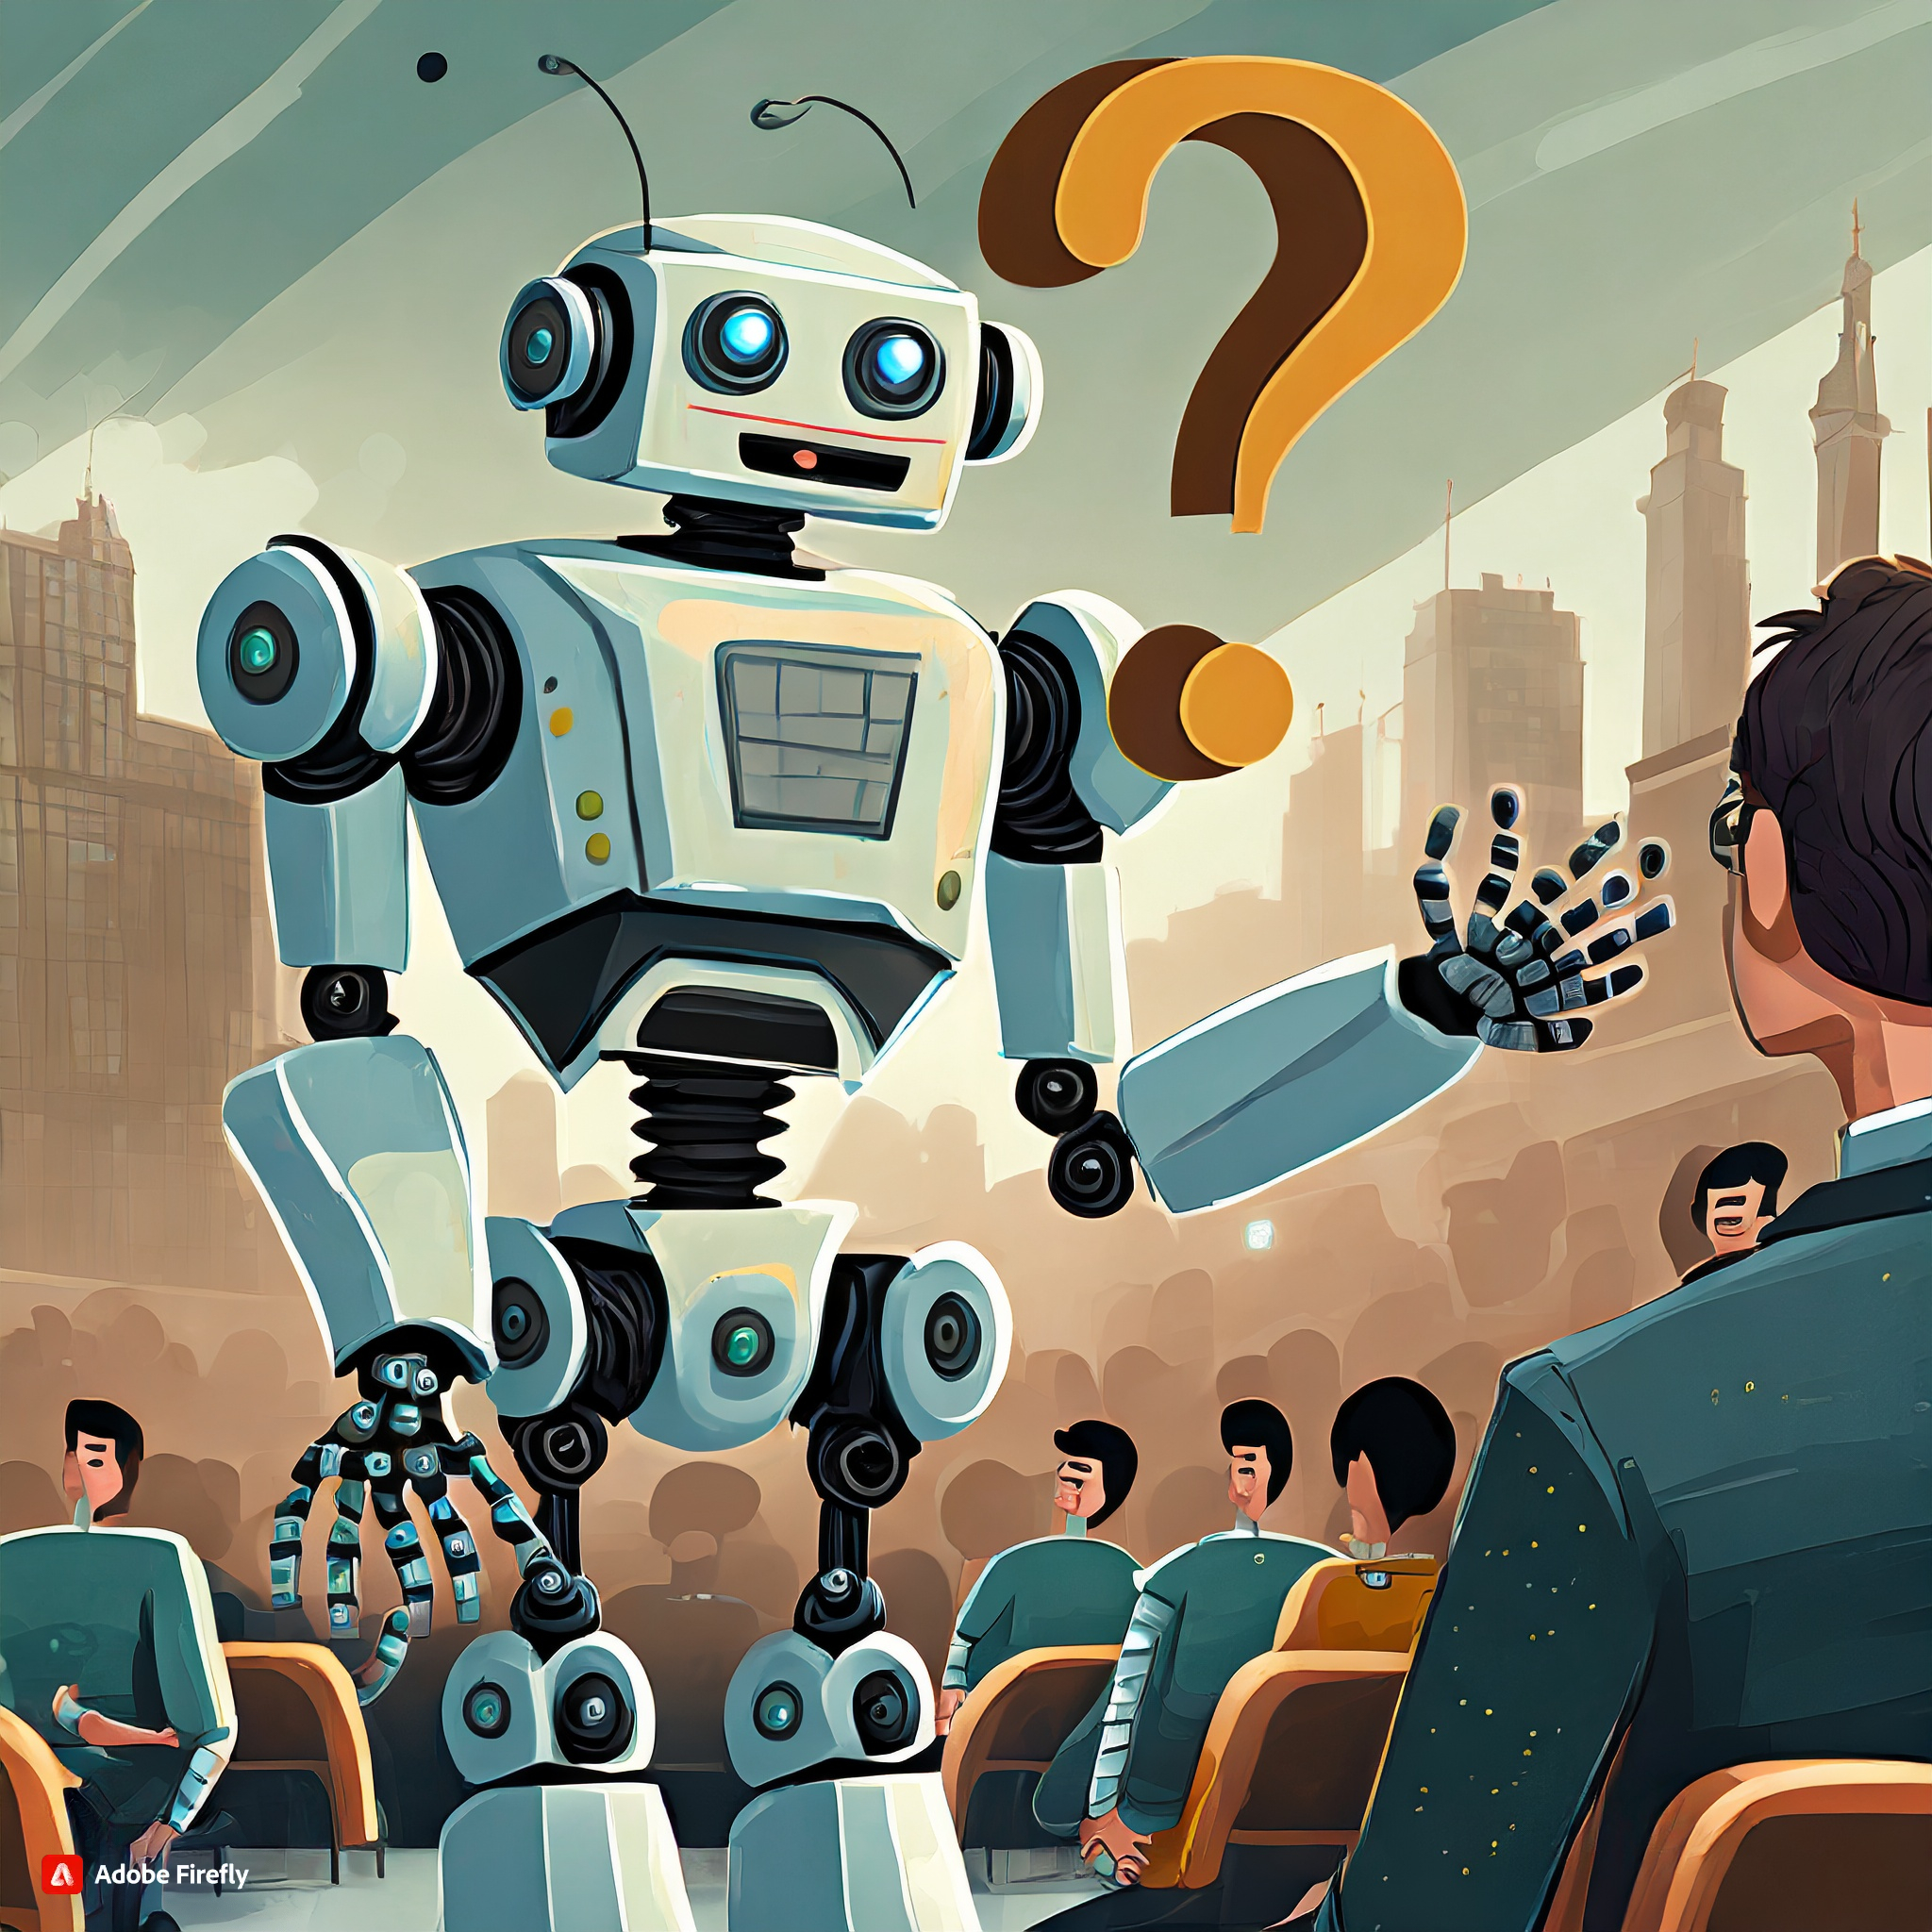
\includegraphics[width=.80\textwidth]{imagens/robo_duvida}
	   \end{flushright}
	   \column{.40\textwidth}
		   \begin{itemize}
		   \item Com dúvidas ?
		   \item Alguma discussão ?
		   \item Algum comentário ?
		   \item Jogando tomates!?
		   \end{itemize}
	\end{columns}
\end{frame}


\end{document}

